\chapter{Einführung in Google Fusion Tables}

\section{Was ist Google Fusion Tables}
Google Fusion Tables wurde am 10. Juni 2009 der Öffentlichkeit zugänglich gemacht\cite{fusion-table-announce}. Das erklärte Ziel dabei war es, die Nutzung einer Datenbank so einfach wie möglich zu machen.

\subsection{Software-as-a-Service (SaaS) / Cloud}
Der Begriff "Software-as-a-Service" (Saas) hat sich in den letzten Jahren etabliert und bezeichnet die Dienstleistung eine Software nicht nur für einen Kunden zu entwickeln, sondern auch gleich deren Betrieb zu übernehmen. Diese gesamthafte Dienstleistung wird dann dem Kunden angeboten, so dass dieser keine eigene Infrastruktur betreiben muss. Die "Cloud" ist die logische  Erweiterung dieses Konzepts, dabei wird der angebotene Dienst transparent auf mehreren Umgebungen und an verschiedenen Lokationenn angeboten. Dies soll zum einen eine hohe Erreichbarkeit gewährleisten, zum anderen kann ein Anbieter dadurch sehr leicht skalieren. \todo[inline]{Quellenverweis}

\subsection{Datenbank in der Cloud}
Google Fusion Tables schafft das Problem der Erreichbarkeit einer Datenbank ab. Fusion Tables sind dezentral in der Cloud gespeichert und dort lassen sie sich einfach vertikal skalieren. Die momentanen geltenden Limiten der Datenbank sind 250MB Speicher für eine Tabelle, 25'000 Abfragen pro Tag und Benutzer sowie 100'000 Elemente, die gleichzeitig auf der Karte dargestellt werden können. Allgemein werden bei Abfragen nur die ersten 100'000 Resultate als Antwort zurückgeliefert. Diese Einschränkungen können Kunden mit Google Maps Premier auf Anfrage verändern. \cite{fusion-tables-geo-limits}

\subsection{Kollaboration und Nutzung von (ver-)öffentlichen Daten}
Der Gedanke der Cloud lässt sich abseits vom technischen noch weiterdenken. Durch die allgemeine Verfügbarkeit der Fusion Tables Datenbank, lassen sich die dort eingetragenen Daten mit anderen Benutzern oder gar der Öffentlichkeit teilen. Es gibt sogar eine eigene Suche für öffentliche Tabellen.\cite{fusion-tables-search} Tabellen können dann mit anderen Tabellen gemerged werden, wodurch die Vereinigung der Daten wiederum neue Möglichkeiten zur Nutzung der Daten ermöglicht. Eine öffentlich zugängliche Tabelle mit Länderpolygonen lässt sich so beliebig oft gebrauchen, um Daten mit Ländern zu verknüpfen und diese dann auf einer Karte darzustellen.

Diese passive Kollaboration ermöglicht es auf eine breite Palette an öffentlichen bzw. veröffentlichten Daten zurückzugreifen. Via Import lassen sich auch andere bereits bestehende Daten mit Fusion Tables nutzen. Unterstützt sind dabei Tabellen (via Google Spreadsheet) und KML Dateien. Mit unserem im Kapitel \ref{converter-build} vorgestellten Build lassen sich eine breite Palette von Dateinformaten in Google Fusion Tables importieren.

Um aktiv zu kollaborieren bieten hat Google auch einige Features angedacht. So ist es möglich einzelne Records oder gar Zellen in der Tabelle zu kommentieren, sofern man die nötigen Berechtigungen dafür hat. Falls man Daten von mehreren Lieferanten verwalten lassen will, kann eine Partei eine Tabelle erstellen und verschiedene Views darauf erstellen, welche jeweils von den verschiedenen Datenlieferanten gepflegt werden. Durch entsprechend gesetzte Berechtigungen kann so jeder seine Daten zum ganzen Beitragen, ohne Zugriff auf die Daten aller anderen Lieferanten zu erlangen. Einzig der Besitzer der Tabelle hat den kompletten Überblick. Google hat als Beispiel für diesen Use Case die Applikation "Flu Vaccine Finder" erstellt, welche es den Anbietern von Grippeimpfungen ermöglicht ihre Lokale selbstständig zu erfassen und verwalten.\cite{data-gathering}


\section{SQL API}
\label{sql-api}
Das SQL API bietet eine Schnittstelle mit welcher man mit SQL-ähnlichen Befehlen Daten aus Google Fusion Tables abfragen oder verändern kann. Sie verfügt bereits über eine grosse Palette an möglichen Befehlen\footnote{Befehlsreferenz: \url{https://developers.google.com/fusiontables/docs/developers_reference}}. Die SQL-Befehle werden als Parameter in folgender Form an das API übergeben:

\url{https://www.googleapis.com/fusiontables/<apiVersion>/query?sql=<statement>}

Lesende Zugriffe (\inlinecode{SELECT}, \inlinecode{SHOW TABLES}, \inlinecode{DESCRIBE}) werden dabei als \inlinecode{GET}-Request geschickt, schreibende Zugriffe (\inlinecode{CREATE}, \inlinecode{DROP}, \inlinecode{INSERT}, \inlinecode{UPDATE}, \inlinecode{DELETE} mit der \inlinecode{POST}-Methode. Um Daten zu schreiben und für den Zugriff auf private Tabelle ist eine Authentifizierung (siehe Abschnitt \ref{oauth}) mit OAuth nötig.

\begin{longtable}{|l|p{11.5cm}|}
\hline 
\textbf{Befehl} & \textbf{Beschreibung} \\ 
\hline 
\inlinecode{SHOW TABLES} & Abfrage aller Tabellen des angemeldeten Benutzers \\ 
\hline 
\inlinecode{DESCRIBE} & Bezeichnung und Datentypen aller Spalten in einer Tabelle \\ 
\hline 
\inlinecode{CREATE TABLE} & Erstellen einer neuen Tabelle \\ 
\hline 
\inlinecode{CREATE VIEW} & Erstellen einer View auf Grundlage einer bestehenden Tabelle \\ 
\hline 
\inlinecode{SELECT} & Selektieren von Daten einer Tabelle \\ 
\hline 
\inlinecode{INSERT} & Neue Zeile zu einer Tabelle hinzufügen \\ 
\hline 
\inlinecode{UPDATE} & Daten in einer Tabelle verändern \\ 
\hline 
\inlinecode{DELETE} & Daten aus einer Tabelle löschen \\ 
\hline 
\inlinecode{DROP TABLE} & Löschen einer Tabelle \\ 
\hline 
\end{longtable}

\subsection{Spatial-Queries}
\label{sqlapi-spatialqueries}
Die FusionTablesLayer bieten zudem eine Reihe von speziellen ortsabhängigen Abfrage-Möglichkeiten, welche in der folgenden Tabelle dokumentiert sind.

\begin{longtable}{|p{4cm}|p{11cm}|}
\hline 
\textbf{Spatial Keyword} & \textbf{Beschreibung} \\ 
\hline 
ST{\_}INTERSECTS( {\textless}location{\_}column{\textgreater}, {\textless}geometry{\textgreater} ) & Kann als Bedingung in der WHERE-Klausel des Statements verwendet werden.

Liefert alle Zeilen zurück, welche sich innerhalb der definierten Geometrie \emph{{\textless}geometry{\textgreater}} befinden.

\begin{itemize}
\item Als \emph{{\textless}location{\_}column{\textgreater}} muss eine Spalte der Tabelle angegeben werden, welche den Typ \emph{location} hat.
\item Als \emph{{\textless}geometry{\textgreater}} kann entweder ein \emph{CIRCLE} oder ein \emph{RECTANGLE} verwendet werden. 
\end{itemize}

\textit{Hinweis: ST{\_}INTERSECTS und ST{\_}DISTANCE dürfen nicht zusammen im gleichen Statement verwendet werden.} \\ 
\hline 
ST{\_}DISTANCE( {\textless}location{\_}column{\textgreater}, {\textless}coordinate{\textgreater} ) & Kann als Bedingung in der ORDER BY-Klausel des Statements verwendet werden.

Liefert die Datensätze sortiert nach der Distanz zur angegebenen Koordinate \emph{{\textless}coordinate{\textgreater}} zurück.

\begin{itemize}
\item Als \emph{{\textless}location{\_}column{\textgreater}} muss eine Spalte der Tabelle angegeben werden, welche den Typ \emph{location} hat.
\item Die \emph{{\textless}coordinate{\textgreater}} stellt die Koordinate dar, zu welcher der Abstand gemessen werden soll. 
\end{itemize}

\textit{Hinweis: ST{\_}INTERSECTS und ST{\_}DISTANCE dürfen nicht zusammen im gleichen Statement verwendet werden.} \\ 
\hline 
CIRCLE( {\textless}coordinate{\textgreater}, {\textless}radius{\textgreater} ) & Wird verwendet, um einen Kreis von der angegebenen Koordinate \emph{coordinate} mit den Radius \emph{radius} zu erhalten. \\ 
\hline 
POLYGON( {\textless}coordinate{\_}1{\textgreater}, {\textless}coordinate{\_}2{\textgreater}, ... ) & Wird verwendet um ein Polygon bestehend aus den angegebenen Koordinaten \emph{coordinate{\_}x} zu erhalten. \\ 
\hline 
RECTANGLE( {\textless}coordinate{\_}1{\textgreater}, {\textless}coordinate{\_}2{\textgreater} ) & Wird verwendet um ein Rechteck mit den Ecken \emph{coordinate{\_}1} (links oben) und \emph{coordinate{\_}2} (rechts unten) zu erhalten. \\ 
\hline 
\end{longtable} 

\section{Client Libraries}
Google bietet zum API bereits auch Client Libraries in den Sprachen PHP und Phyton an. Da unserer Applikation aber möglichst nur in Javascript implementiert werden soll erstellten wir uns eine Javascript Library zur Verwendung des SQL APIs.

Durch die Same origin policy\footnote{Die Same-Origin-Policy (SOP) ist ein Sicherheitskonzept, das es JavaScript und ActionScript nur dann erlaubt, auf Objekte einer anderen Webseite zuzugreifen, wenn sie aus derselben Quelle (Origin) stammen.\cite{sop} }, welche es uns daran hinderte AJAX-Requests direkt auf das Google API abzusetzen, mussten wir zuerst nach Lösungen für dieses Problem suchen. Wir wollten es verhindern einen PHP-Server dazwischen zu schalten, welcher uns die Abfragen abnimmt.

So fanden wir in den Google Groups ein inoffizielles JSONP API, welches es erlaubt AJAX-Requests auch über die eigene Domäne hinweg zu senden. Dies funktioniert jedoch nur für lesende Zugriffe. Für alle schreibenden Zugriffe mussten wir eine Umgeheungslösung bauen, bei der die Requests über unseren Webserver geschleust wurden. Damit konnten wir die Same-Origin-Policy umgehen. Mit Hilfe des Trusted Tester API (Siehe Abschnitt~\ref{trusted-tester-api}) haben wir schlussendlich dann aber doch noch eine Lösung gefunden, welche direkt im Browser läuft und somit nicht auf Server-Code angewiesen ist.

\section{Trusted Tester API}
\label{trusted-tester-api}
Es gibt derzeit zwei verschiedene Versionen des APIs: eine frei öffentlich zugängliche und das sogenannte "Trusted Tester API", welche derzeit im Beta-Stadium ist und ausgewählten Personen zur Verfügung steht. Als wir im Sprint 2 davon erfahren haben, haben wir uns für einen Zugang beworben, welchen wir dann auch erhalten haben.

Das Trusted Tester API bietet einige Neuerungen zur alten Schnittstelle. Es handelt sich bei diesem API um eine Vorabversion der neuen Schnittstelle, welche zukünftig ebenfalls der Öffentlichkeit zur Verfügung stehen soll. Neben dem API gibt es auch eine zugehörige Mailingsliste, auf der die Entwickler von Google Fragen beantworten und Tipps geben, aber auch dazu aufrufen, dass neue API ausgiebig zu testen.

Zu den Neuerungen des neuen APIs gehört, dass es auch eine REST-Schnittstelle\cite{rest} bekommen hat. Damit ist es zum einen möglich Tabelleninformationen abzufragen als auch ganz klassisch CRUD-Operationen auf dem API auszuführen. Da wir uns bemüht haben unsere Beispiele möglichst ohne Server-Code zu schreiben, konnten wir besonders davon profitieren, mit dem neuen API POST-Requests abzuschicken und somit endlich auch Schreiboperationen direkt via Browser zu unterstützen. \todo{SOP und Relay-Service, ist das irgendwo schon dokumentiert?}

\subsection{Übersicht}
Alle Request an das REST-API haben die folgende Form:
\url{https://www.googleapis.com/fusiontables/<apiVersion>/<resourcePath>?<parameters>}

Folgende Ressourcen sind derzeit unterstützt:
\begin{itemize}
	\item Table
	\item Column
	\item Template
	\item Style
\end{itemize}

Eine Row oder Query Ressource fehlt noch. Um Abfragen zu machen muss nach wie vor das SQL API (siehe Abschnitt \ref{sql-api}) verwendet werden.

\begin{longtable}{|l|p{6cm}|p{7cm}|}
\hline 
\textbf{Operation} & \textbf{Beschreibung} & \textbf{HTTP Mapping} \\ 
\hline 
list & Alle Ressourcen eines Typs auflisten & \inlinecode{GET} auf einem Ressource-Typ\\ 
\hline 
get	 & Eine spezifische Ressource holen	& \inlinecode{GET} auf einer Ressource\\
\hline 
insert & Eine neue Ressource einfügen (kreiert eine neue Ressource) & \inlinecode{POST} auf einem Ressource-Typ (mit Daten um eine neue Ressource zu erstellen)\\
\hline 
update & Aktualisieren einer bestehenden Ressource & \inlinecode{PUT} auf einer Ressource (mit Daten um die Ressource zu aktualisieren)\\
\hline 
delete & Löschen einer Ressource & \inlinecode{DELETE}  auf einer Ressource\\
\hline 
\end{longtable}

\subsection{Migration zum neuen API}
Um zum neuen API zu migrieren müssen einige Dinge beachtet werden.


\subsection{Bugs und Austausch mit den Google Entwicklern}

\section{Geocodierung}
Ein grosser Vorteil der Google Fusion Tables ist die automatische 
\gls{Geocodierung} von Standortdaten. Sobald eine neue Zeile zu einer Tabelle hinzugefügt wird, werden alle Zellen vom Typ \emph{Location} einem eindeutigen Standort auf der Karte zugewiesen. Ist dies nicht möglich, da beispielsweise eine Adresse in mehreren Orten vorkommen kann, bleibt die Zelle gelb hinterlegt.
 
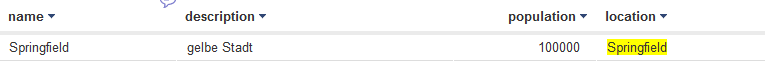
\includegraphics[scale=0.75]{images/geocoding_failed.png}

Diese geocodierten Standorte werden in der Tabelle hinterlegt sind aber mit den SQL API nicht selektierbar. Man müsste also für jede Zeile die man als Resultat erhält die Geocodierung manuell vornehmen, was sich negativ auf die Ladezeit der Karte auswirken würde.
Es gibt verschiedene Dienste, welche eine solche Geocodierung von Standortdaten anbieten. Die meisten davon haben aber eine Begrenzung der möglichen Anfragen pro Tag.

\begin{longtable}{|l|p{1.9cm}|p{7.3cm}|}
\hline 
\textbf{Anbieter} & \textbf{Anfragen pro Tag} & \textbf{URL} \\ 
\hline 
Google Maps Geocoding API & 2500 & \url{https://developers.google.com/maps/documentation/geocoding/?hl=de} \\ 
\hline 
Yahoo! PlaceFinder API & 50000 & \url{http://developer.yahoo.com/geo/placefinder/} \\ 
\hline 
MapQuest Geocoding API & keine Begrenzung & \url{http://developer.mapquest.com/web/products/dev-services/geocoding-ws} \\ 
\hline 
\end{longtable} 

Wie man sieht erreicht man mit diesen Diensten beim Arbeiten mit grossen Datenmengen schnell die Grenzen.

\section{Google Maps API - FusionTablesLayer}
\label{gmap-api-fusiontableslayer}
Google bietet von Haus aus aber bereits eine Fusion Table-Integration im Google Maps API V3 an. Damit ist es möglich Fusion Tables als eigenständige Layer direkt auf der Karte darzustellen.
Die Möglichkeiten dieser Layer sind noch stark eingeschränkt aber die grundlegenden Funktionalitäten für das Arbeiten mit Geodaten sind bereits vorhanden.

So ist es möglich Abfragen mit WHERE-Conditions einzuschränken oder die Stile des Layers selbst zu bestimmen. Man kann beispielsweise Flächen mit Zeckengebieten je nach Intensität des Befalls anders einfärben.

\subsection{Karten-Stile}
Die FusionTablesLayer bieten ein abfragebasiertes Styling der Ebene an. Damit ist es möglich Flächen oder Linien farblich hervorzuheben oder Custom-Icons für Markierung zu verwenden. Zu jedem Stil kann man eine Einschränkung festlegen, welche bestimmt, ob dieser für den aktuellen Datensatz angewendet wird oder nicht. Die Einschränkung entspricht grundsätzlich einer WHERE-Condition in der Abfrage.

\emph{Hinweis: Kann ein Datensatz keinem Stil zugewiesen werden, da er in keine Einschränkung passt, erhält er den letzten definierten Stil.}

\subsubsection{Beispiel eines Stils:}
\lstset{language=JavaScript}
\begin{lstlisting}
styles: [{
	polygonOptions: {
		fillColor: "#00FF00", // gruen
		fillOpacity: 0.3
	}
}, {
	where: "birds > 300",
	polygonOptions: {
		fillColor: "#0000FF" // blau
	}
}]
\end{lstlisting}

In diesem Beispiel\footnote{Quelle: \url{https://developers.google.com/maps/documentation/javascript/layers?hl=de-DE\#fusion_table_styles} (Stand: 21.05.2012)} werden alle Polygone der Tabelle, welche in der Spalte \emph{birds} eine Zahl grösser als 300 eingetragen haben, \emph{blau} eingefärbt. Die restlichen Polygone erhalten eine \emph{grüne} Färbung mit einer Deckkraft von 30\%.

\subsubsection{Einschränkungen}
\label{fusiontableslayer-styles-restrictions}
Das Google Maps API hat momentan folgende Einschränkungen bezüglich den Ebenenstilen definiert.

\begin{itemize}
\item Auf einer Karte können maximal 5 FusionTablesLayer gleichzeitig angezeigt werden
\item Stile können dabei nur für eine dieser Ebenen angewendet werden
\item Zudem dürfen für diese Ebene maximal 5 Stile definiert sein
\end{itemize}

\subsection{Heatmaps}
Ein weiteres Feature der Fusion Table-Ebenen ist die Möglichkeit die Daten der Tabelle direkt als Heatmap darzustellen. Dabei werden die Daten automatisch nach der Häufigkeit der Vorkommnisse an einem Ort anders eingefärbt. Der verwendete Farbverlauf geht dabei von Grün (für wenig Daten) bis Rot (für viele Daten).

\begin{figure}[!h]
	\centering
	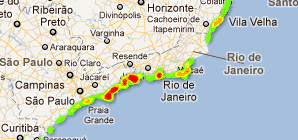
\includegraphics{images/gmap_fusiontableslayer_heatmap.png}
	\caption{Daten als Heatmap mit FusionTablesLayer}
	\label{fusiontableslayer-heatmap}
\end{figure}

Leider sind momentan die Konfigurationsmöglichkeiten der Heatmap auf ein Minimum beschränkt. Es ist lediglich möglich zu definieren, ob die Heatmap angezeigt werden soll oder nicht. Eine Legende lässt sich beispielsweise nicht anzeigen. So kann man nicht genau sagen, welche werte nun hinter der grünen oder der roten Farbe stecken. Zudem lassen sich diese Farben auch nicht anpassen.

\subsection{Performance}
Der grösste Vorteil der Fusion Table-Ebenen steckt aber nicht zwingend in den sichtbaren Features. Man findet ihn wohl eher darin, dass die Geocodierungen der Standort-Daten direkt aus der Tabelle gelesen werden und nicht manuell vom Client abgefragt werden müssen. Dadurch kann die Ebene komplett auf den Servern von Google aufbereitet werden. Der Client muss die erhaltenen Daten lediglich noch darstellen. Der Vorteil davon wird durch das folgende Diagramm\footnote{Quelle: \url{http://www.google.com/events/io/2011/sessions/managing-and-visualizing-your-geospatial-data-with-fusion-tables.html} (Stand: 17.05.2012)} schnell ersichtlich.

\begin{figure}[htbp]
	\centering
	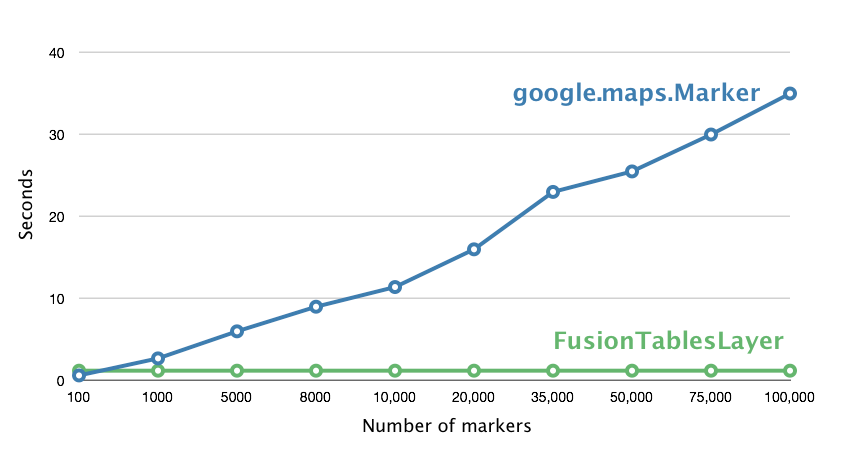
\includegraphics[scale=0.5]{images/gmap_fusiontableslayer_vs_markers.png}
	\caption{FusionTablesLayer verglichen mit Markers}
	\label{fusiontableslayer-compare_markers}
\end{figure}

Die Zeit für das Rendering der Karte bleibt demnach bei der Verwendung von Fusion Table-Ebenen konstant und somit unabhängig von der Anzahl Markierungen, welche gesetzt werden müssen. Der Rechenaufwand, der für das Erstellen der Javascript Marker-Objekte verwendet werden müsste, wird direkt von den Google Servern übernommen und das Resultat als Bild zum Client gesendet. Daraus resultiert die konstante Zeit, welche für die Anfrage zum Server und für das Senden der Antwort zum Client verwendet wird.

\subsection{Nachteile}
\subsubsection{Freigabe der Tabelle}
Ein grosser Nachteil der Fusion Table-Ebenen besteht aber darin, dass die verwendeten Fusion Tables als  \emph{öffentlich} markiert sein müssen, um diese auf einer Karte darzustellen. Sprich jeder kann die Tabellen anzeigen oder auslesen. Es ist also nicht möglich eine Tabelle mit sensiblen Daten als Fusion Table-Ebene darzustellen.

Von Google wird zur Lösung dieses Problems aber folgendes Vorgehen vorgeschlagen: Man kann für Tabellen mit sensiblen Inhalten eine View erstellen, welche lediglich die öffentlichen Spalten und Zeilen selektiert. Diese View könnte man dann als \emph{öffentlich} markieren und in einer Fusion Table-Ebene verwenden.

Eine Ausnahme dieser Regelung bilden dabei die Maps API Premier Kunden. Diese haben die Möglichkeit eine Fusion Table als \emph{Protectet Map Layer} freizugeben, wodurch sich diese nur in einer definierten Applikation als Ebene einbinden lässt. Die Datenbank bleibt dabei komplett privat und kann nicht ausgelesen werden.

Die Lizenzpreise für Maps API Premier Kunden beginnen bei 10'000\$ pro Jahr und unterscheiden sich je nach Bedürfnis und Verwendung. 

\subsubsection{Anzahl Datensätze in Fusion Table}
Zusätzlich werden lediglich die ersten 100'000 Zeilen der Tabelle gelesen. Alle weiteren Zeilen werden nicht in die Erstellung des Layer einbezogen und somit auch nicht angezeigt.

\subsubsection{Event-Handling auf Fusion Table-Ebenen}
Bislang ist es erst möglich den Klick-Event auf einer Fusion Table-Ebene zu Behandeln. Dieser liefert standardmässig das Template des InfoWindows mit, welches mit dem Klick angezeigt wird. Zudem erhält man die Daten der "angeklickten Zeile" beziehungsweise die zugehörigen Daten des angeklickten Objekts auf der Karte. Man hat die Möglichkeit dieses Template anzupassen bevor das InfoWindow angezeigt wird.

Weitere Events können auf einer Fusion Table-Ebene aber noch nicht behandelt werden. Es ist also nicht möglich beispielsweise ein Objekt auf der Karte bei einem MouseOver-Event anders einzufärben oder ähnliches.

Diese fehlenden Möglichkeiten wurden schon oft von anderen FusionTables-Benutzern bei den Google-Entwicklern angefordert, welche dies ebenfalls als ein wichtiges Feature sehen, dass noch implementiert werden muss.

Als Übergangslösung findet sich bereits eine Custom Library mit dem Namen \emph{Fusion Tips} (\url{http://gmaps-utility-gis.googlecode.com/svn/trunk/fusiontips/docs/examples.html}). Diese legt über die Fusion Table-Ebene eine weitere transparente Ebene. Auf dieser Ebene kann man alle Events, welche das Google Maps API anbietet behandeln (somit auch den MouseOver-Event). Sobald die Maus über die Position eines Elementes auf der Fusion Table fährt, sendet der Event einen Request über das SQL API an die Fusion Table und holt sich die Informationen zu der entsprechenden Zeile. So ist es möglich ein neues Element mit der gleichen Form aber beispielsweise einer anderen Farbe darüber zu legen.

Für den Benutzer entsteht so der Effekt als würde sich die Farbe des gehoverten Elementes ändern.

Die Libary wird in folgendem Blog-Artikel noch sehr gut erklärt: \url{http://csessig.wordpress.com/2012/02/07/multiple-layers-and-rollover-effects-for-fusion-table-maps/}

\section{Google Fusion Table Javascript Library (gftlib-js)}
\label{gftlib-js}
Die Google Fusion Table Javascript Library vereinfacht die Kommunikation mit dem Google Fusion Table SQL API. Sie hilft dabei SQL-Queries zu erstellen und per AJAX an das API zu versenden.

Zur Erstellung der AJAX-Requests werden die \$.get()- und \$.post()-Helpermethoden der jQuery Library in der Version 1.7.1 (Minified) verwendet.

adfasfsadf,

\subsection{Abhängikeiten}
\begin{longtable}{|l|l|p{11.5cm}|}
\hline 
\textbf{Library} & \textbf{Version} & \textbf{Verwendung} \\ 
\hline 
jQuery & 1.7.1-min & AJAX-Requests und weitere Helper-Funktionen \\ 
\hline 
\end{longtable} 

\subsection{Methoden}
\begin{longtable}{|l|p{4.5cm}|p{5cm}|}
\hline 
\textbf{Methode} & \textbf{Beschreibung} & \textbf{Parameter} \\ 
\hline 
execSql(callback, query) & Führt einen SQL-Befehl & callback (Funktion): Callback-Methode welche nach Beendigung der Methode aufgerufen wird. query (String): SQL-Query \\ 
\hline 
execSelect(callback, options) & Führt einen SQL-Abfrage aus & callback (Funktion): Callback-Methode welche nach Beendigung der Methode aufgerufen wird. query (String): SQL-Query \\ 
\hline 
convertToObject(gftData) & Konvertiert das Resultat einer Abfrage in sprechende Objekte & • \\ 
\hline 
\end{longtable} 

\section{Authentifizierung mit OAuth}
\label{oauth}
